\newpage
\section{Resultados}

\subsection{Método para regeneração do clock}

	Foi realizada a montagem do equipamento de acordo com a Figura \ref{fig:m1}, conforme mostram a Figura \ref{fig:f2} e Figura \ref{fig:f4}.

\begin{figure}[H]
	\centering
	\caption{Montagem dos módulos U-2970A e U-2970B.}
	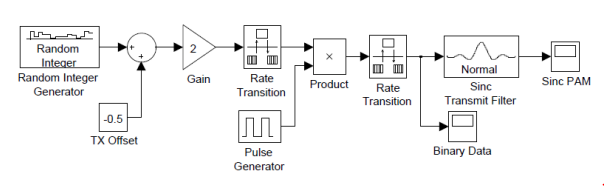
\includegraphics[scale=0.08]{f2}
	
	\small Fonte: Autoria própria.
	\label{fig:f2}
\end{figure}

\begin{figure}[H]
	\centering
	\caption{Montagem do módulo U-2970H.}
	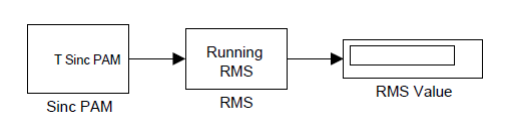
\includegraphics[scale=0.08]{f4}
	
	\small Fonte: Autoria própria.
	\label{fig:f4}
\end{figure}

	Com o osciloscópio na saída NRZ do modulo U02970B e na saída bi-fásica, canais 1 e 2 respectivamente, foi observado um atraso de metade do tempo de bit na saída bi-fase em relação a entrada NRZ.
	
	Com a entrada de dados em 01010000, foi possível observar o comportamento da saída bi-fásica, onde para um bit de entrada 1, a saída corresponde a uma transição do nível lógico alto para o nível lógico baixo no meio do período de bit. Para um bit de entrada 0, a saída corresponde a uma transição do nível lógico baixo para o nível lógico alto, no meio do período de bit, conforme mostra a Figura \ref{fig:f1}. Esse resultado confere com o esperado, pois o primeiro semi-ciclo do período de bit corresponde ao bit de entrada e a segunda metade do período corresponde ao inverso do bit de entrada.
	
	\begin{figure}[H]
		\centering
		\caption{Entrada NRZ (em amarelo) e saída bi-fase (em azul).}
		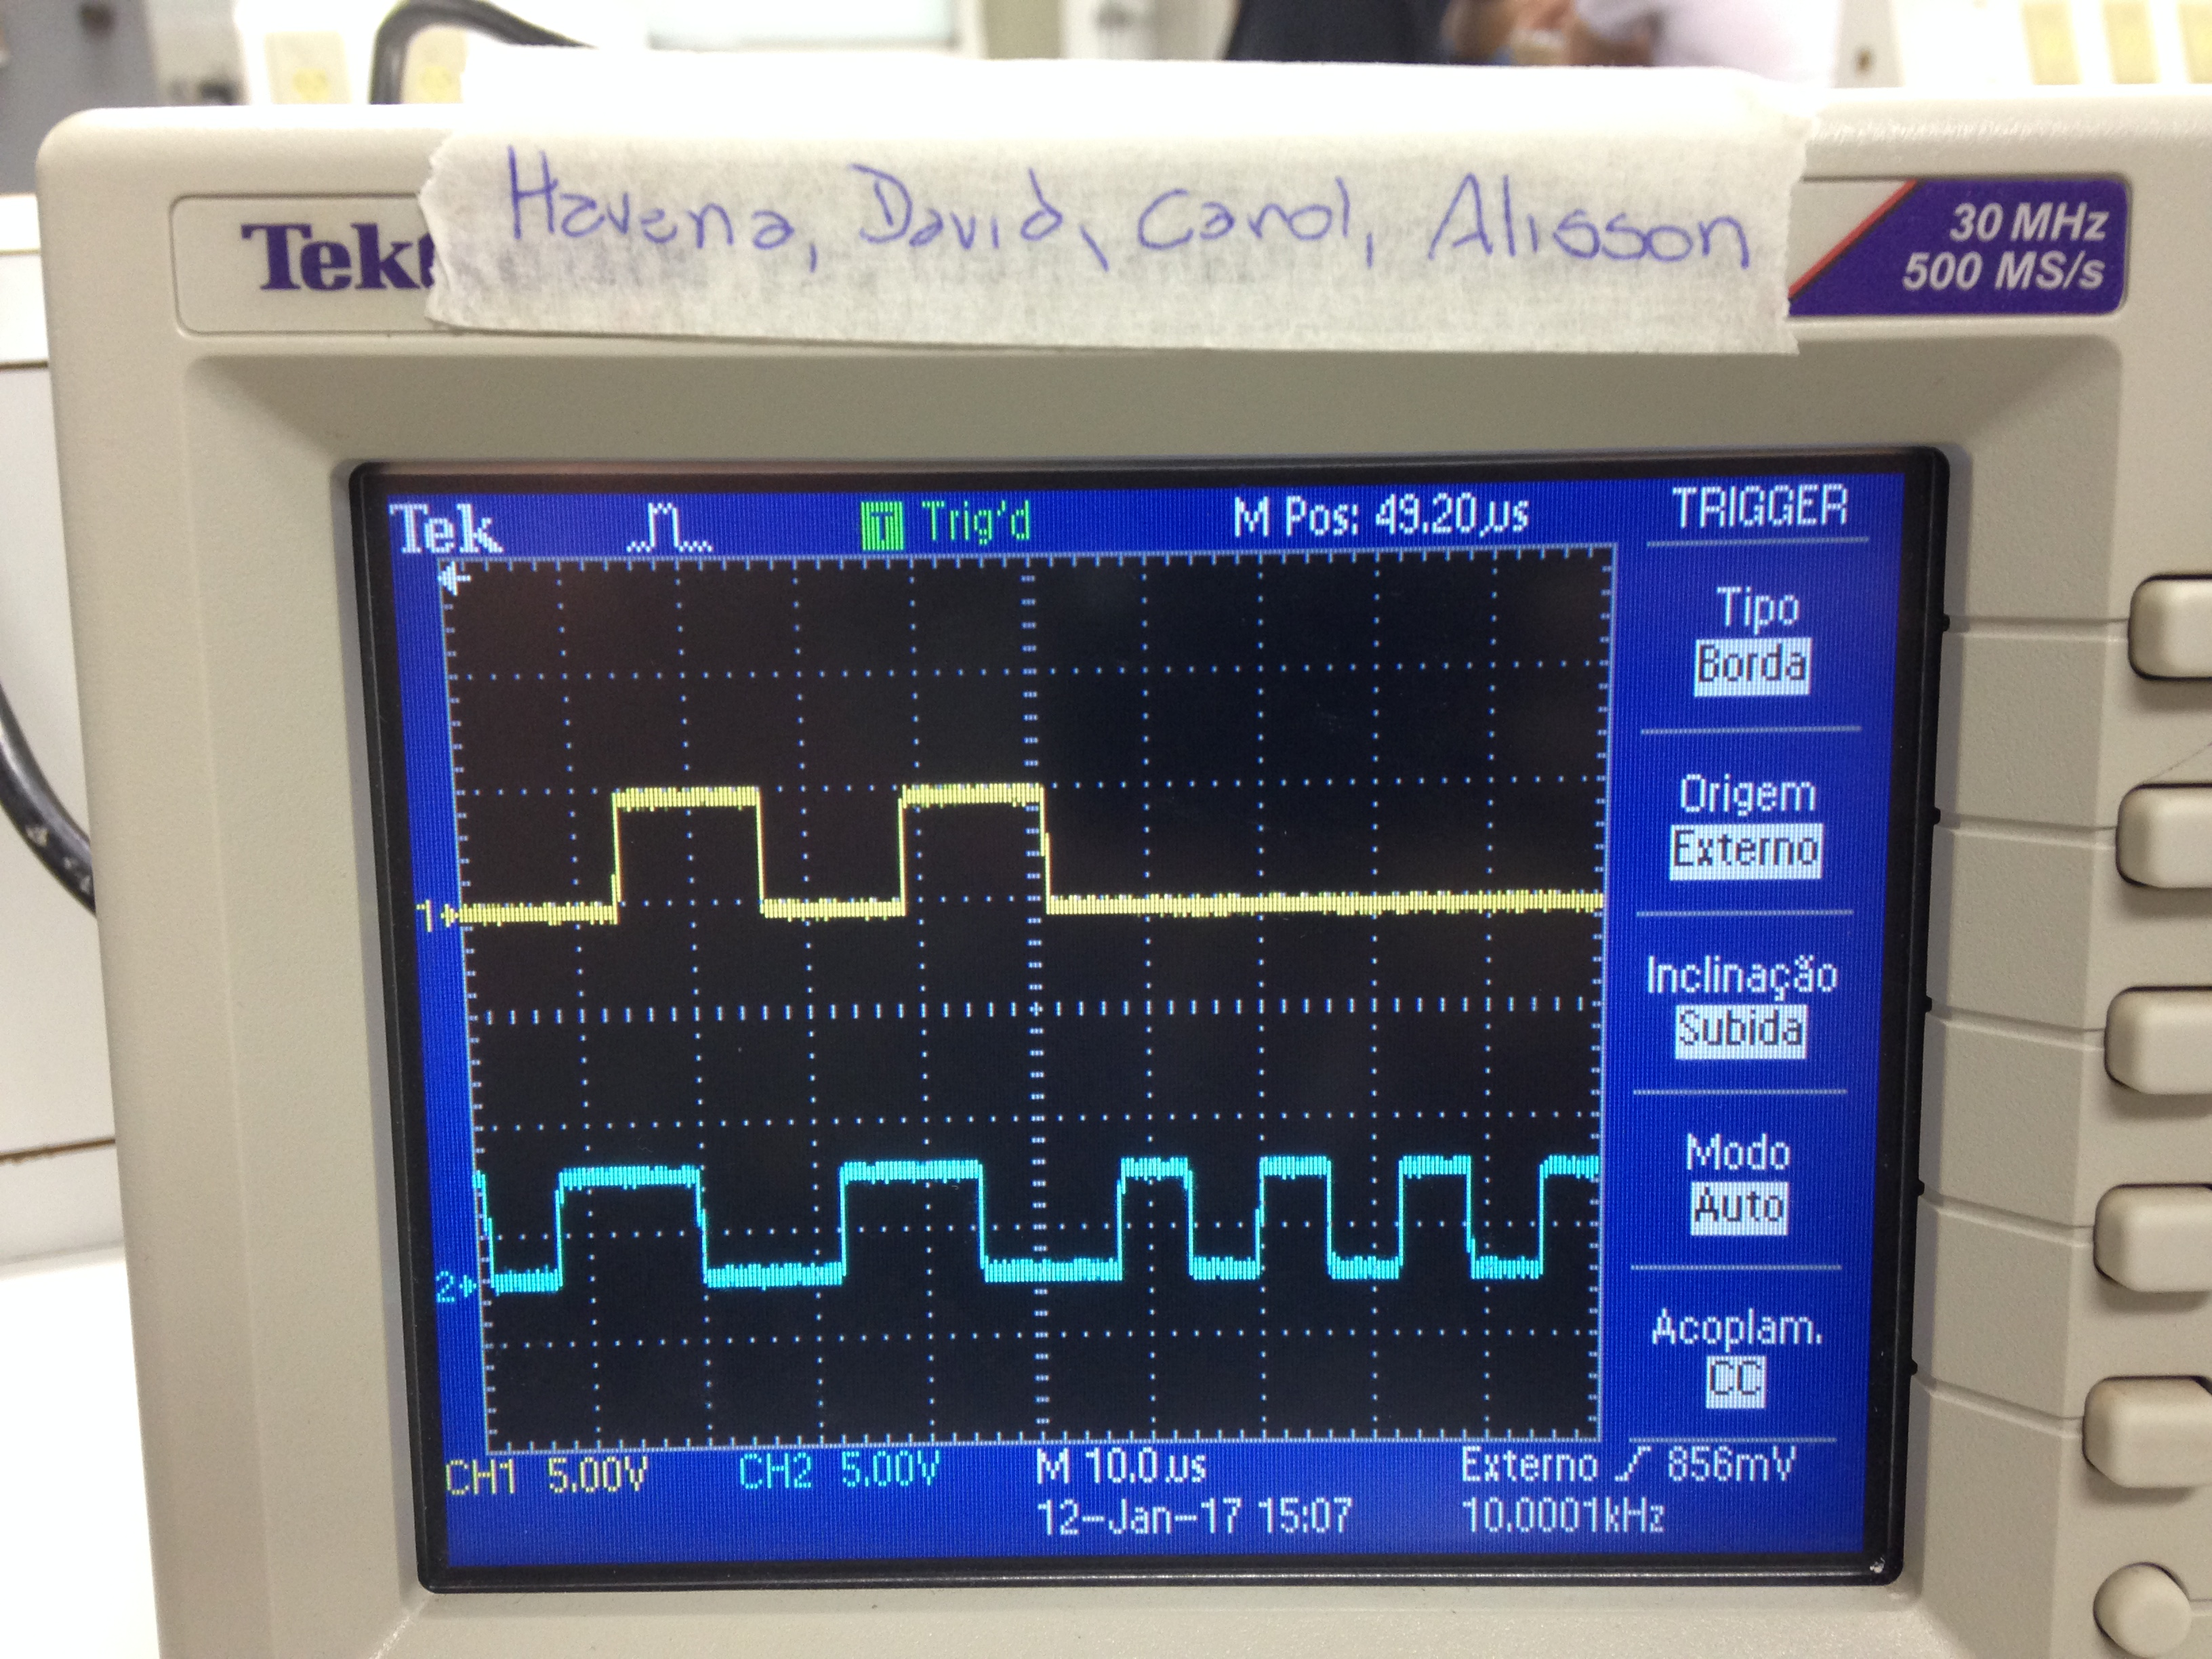
\includegraphics[scale=0.08]{f1}
		
		\small Fonte: Autoria própria.
		\label{fig:f1}
	\end{figure}
	
	Com o canal 1 do osciloscópio na ligação 11 (Figura \ref{fig:f3}), é possível observar que um pulso é gerado a cada transição de estado, garantindo um pulso na metade de cada período de bit. Contudo, o pulso não é garantido ao final do período de bit.
	
		\begin{figure}[H]
			\centering
			\caption{Pulsos na saída do derivador (em amarelo) e saída bi-fase (em azul).}
			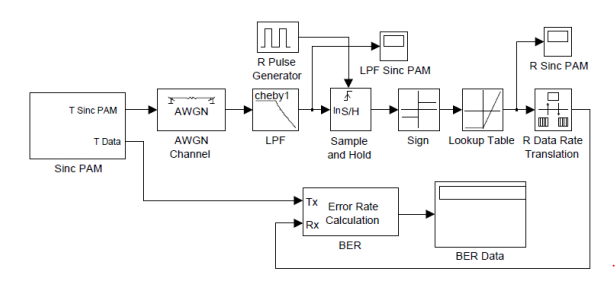
\includegraphics[scale=0.08]{f3}
			
			\small Fonte: Autoria própria.
			\label{fig:f3}
		\end{figure}

\subsection{Recuperação do bit de clock}

	Para verificar a sincronização, a entrada de dados utilizada foi 00000000 e a ligação 1 foi desconectada.
	
	Ao desconectar e reconectar rapidamente a ligação 11, foi observado que o sinal de saída se tornava tudo um ou tudo zero, conforme Figura \ref{fig:f4_2} e Figura \ref{fig:f5}, respectivamente. Ao pressional o botão de sincronização, ou colocar um dos bits de entrada em nível lógico 1, a sincronização foi restaurada.
	
	\begin{figure}[H]
		\centering
		\caption{Saída após desconexão momentânea da ligação 11 (tudo zero).}
		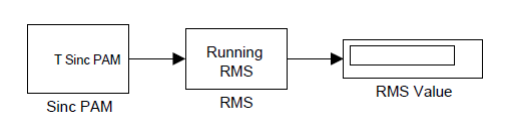
\includegraphics[scale=0.08]{f4}
				
		\small Fonte: Autoria própria.
		\label{fig:f4_2}
	\end{figure}
			
	\begin{figure}[H]
		\centering
		\caption{Saída após desconexão momentânea da ligação 11 (tudo um).}
		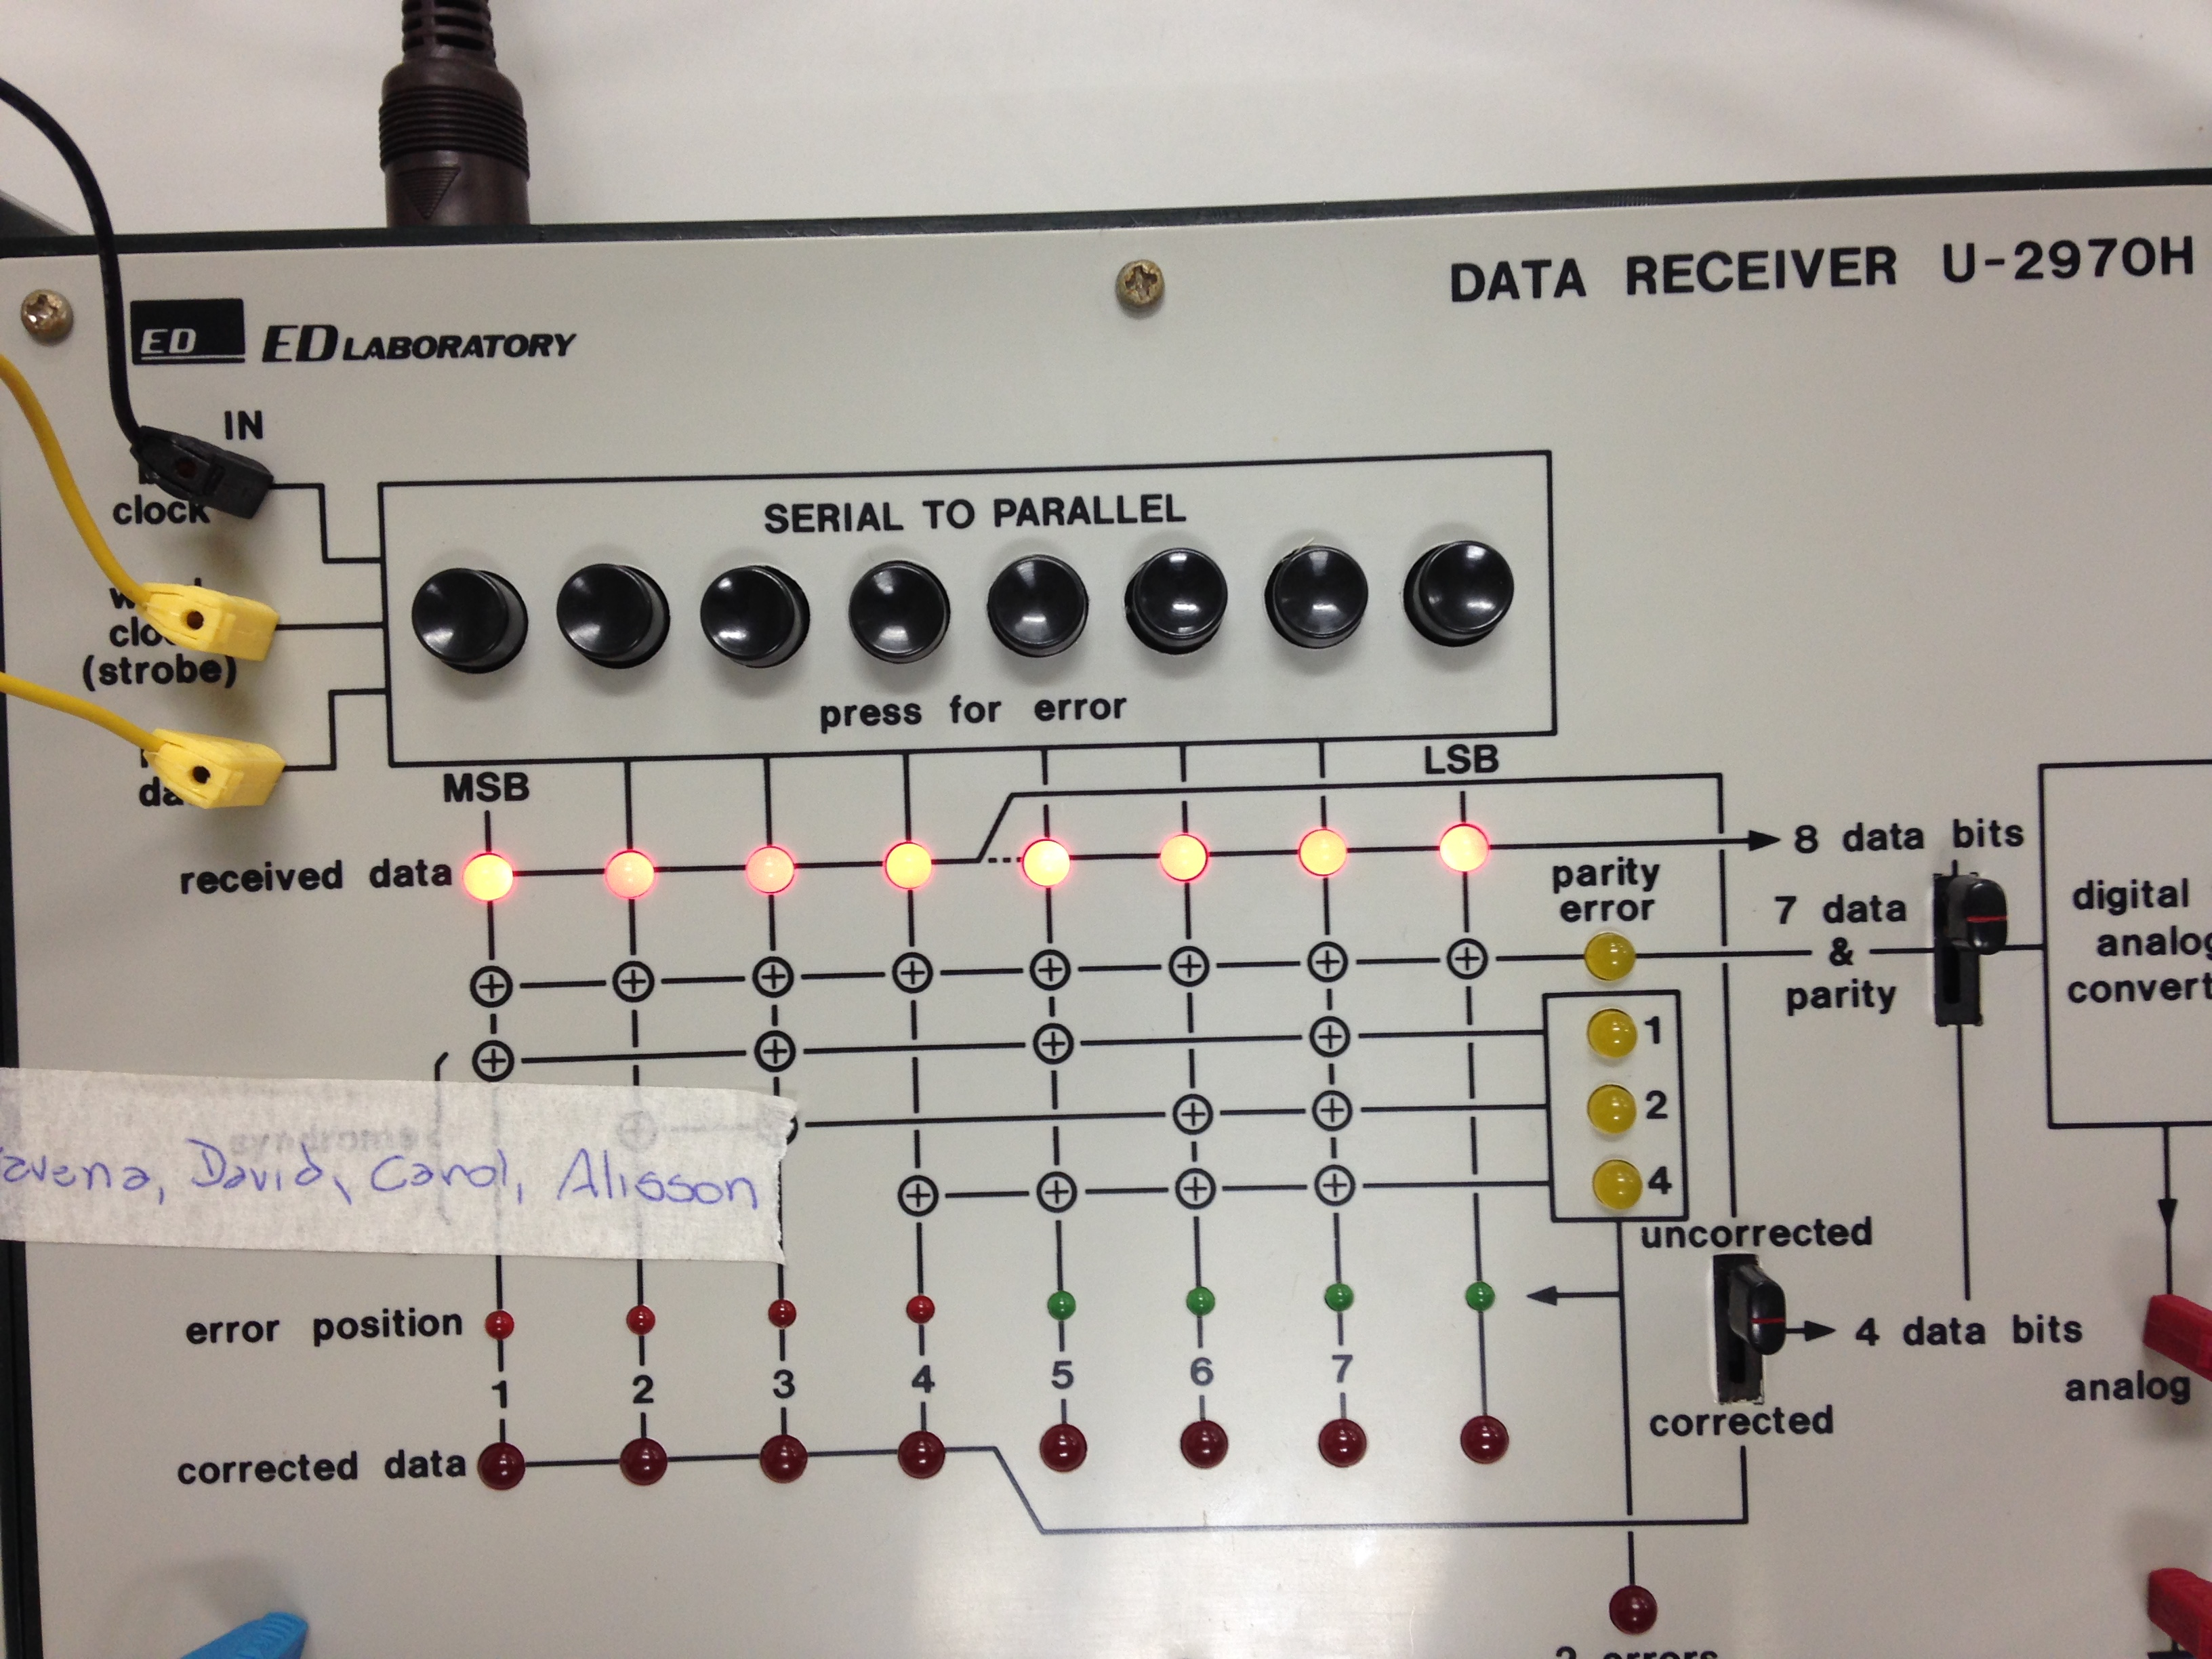
\includegraphics[scale=0.08]{f5}
						
		\small Fonte: Autoria própria.
		\label{fig:f5}
	\end{figure}
	
	Com a ligação 1 restaurada, foi configurada a entrada de dados 01011000 (Figura \ref{fig:f6}), obtendo-se na saída o resultado mostrado na Figura \ref{fig:f7}.
	
	\begin{figure}[H]
		\centering
		\caption{Entrada de dados 01011000.}
		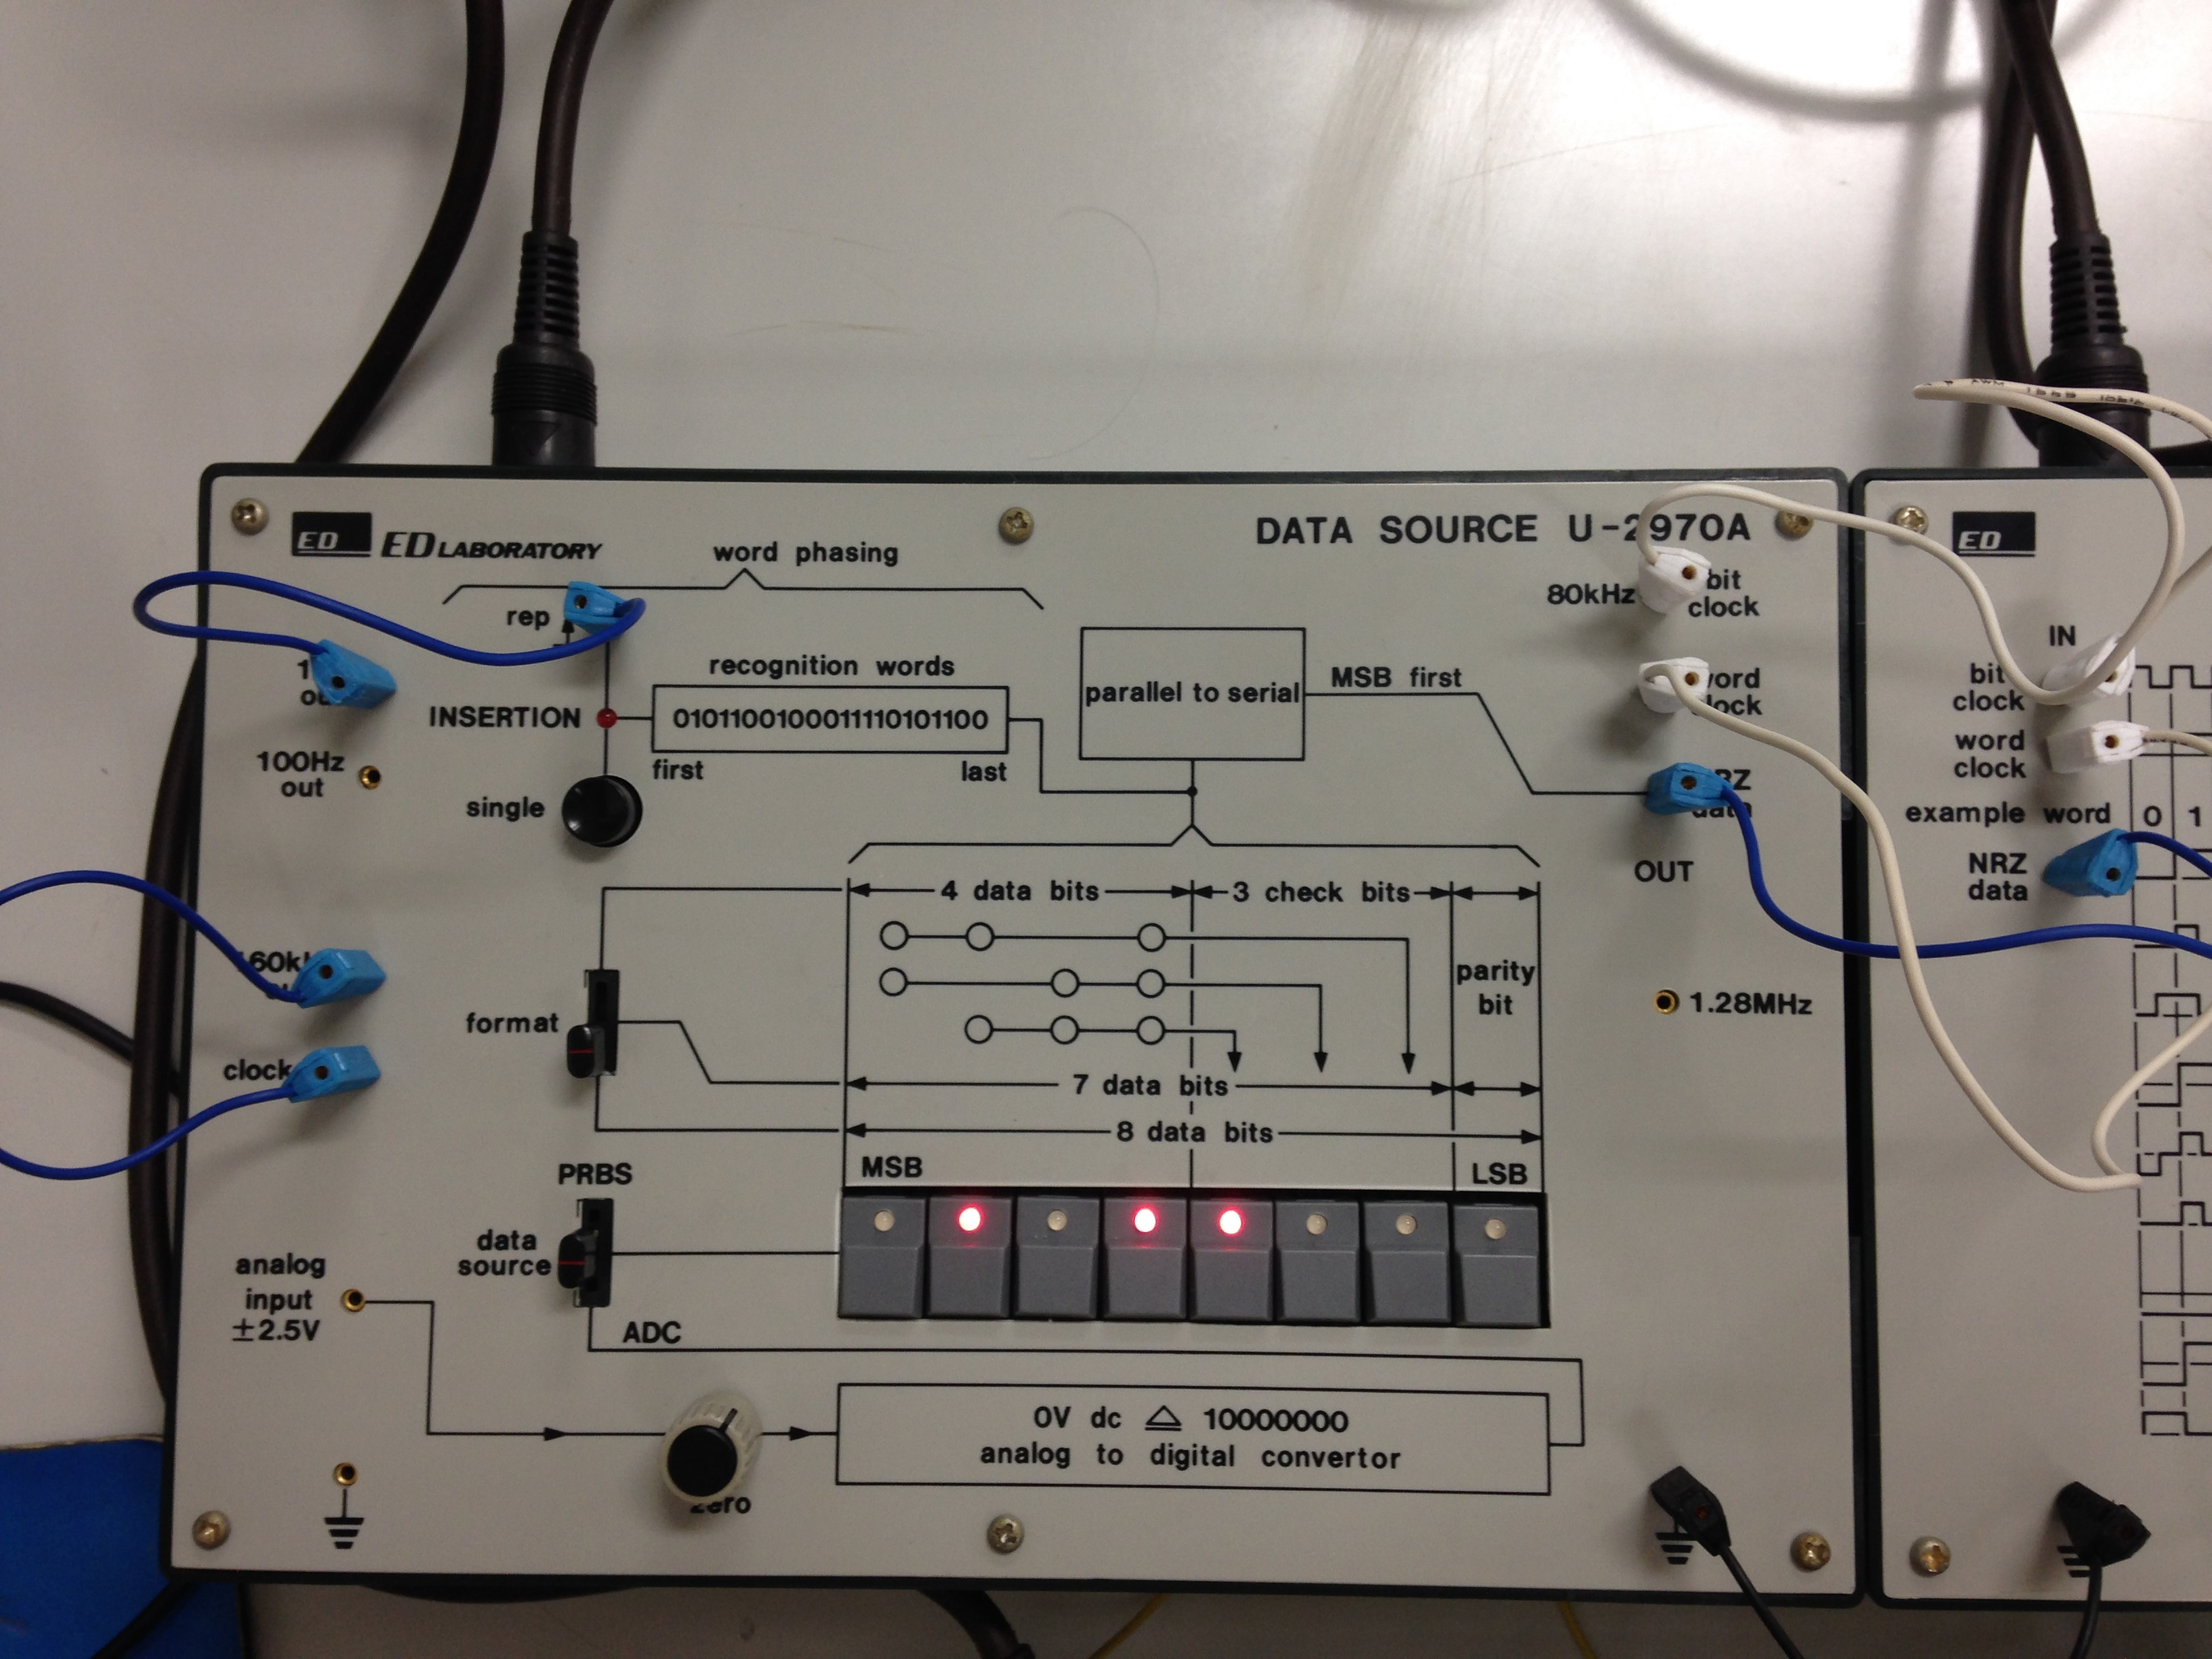
\includegraphics[scale=0.08]{f6}
			
		\small Fonte: Autoria própria.
		\label{fig:f6}
	\end{figure}
	
	\begin{figure}[H]
		\centering
		\caption{Saída para entrada de dados 01011000.}
		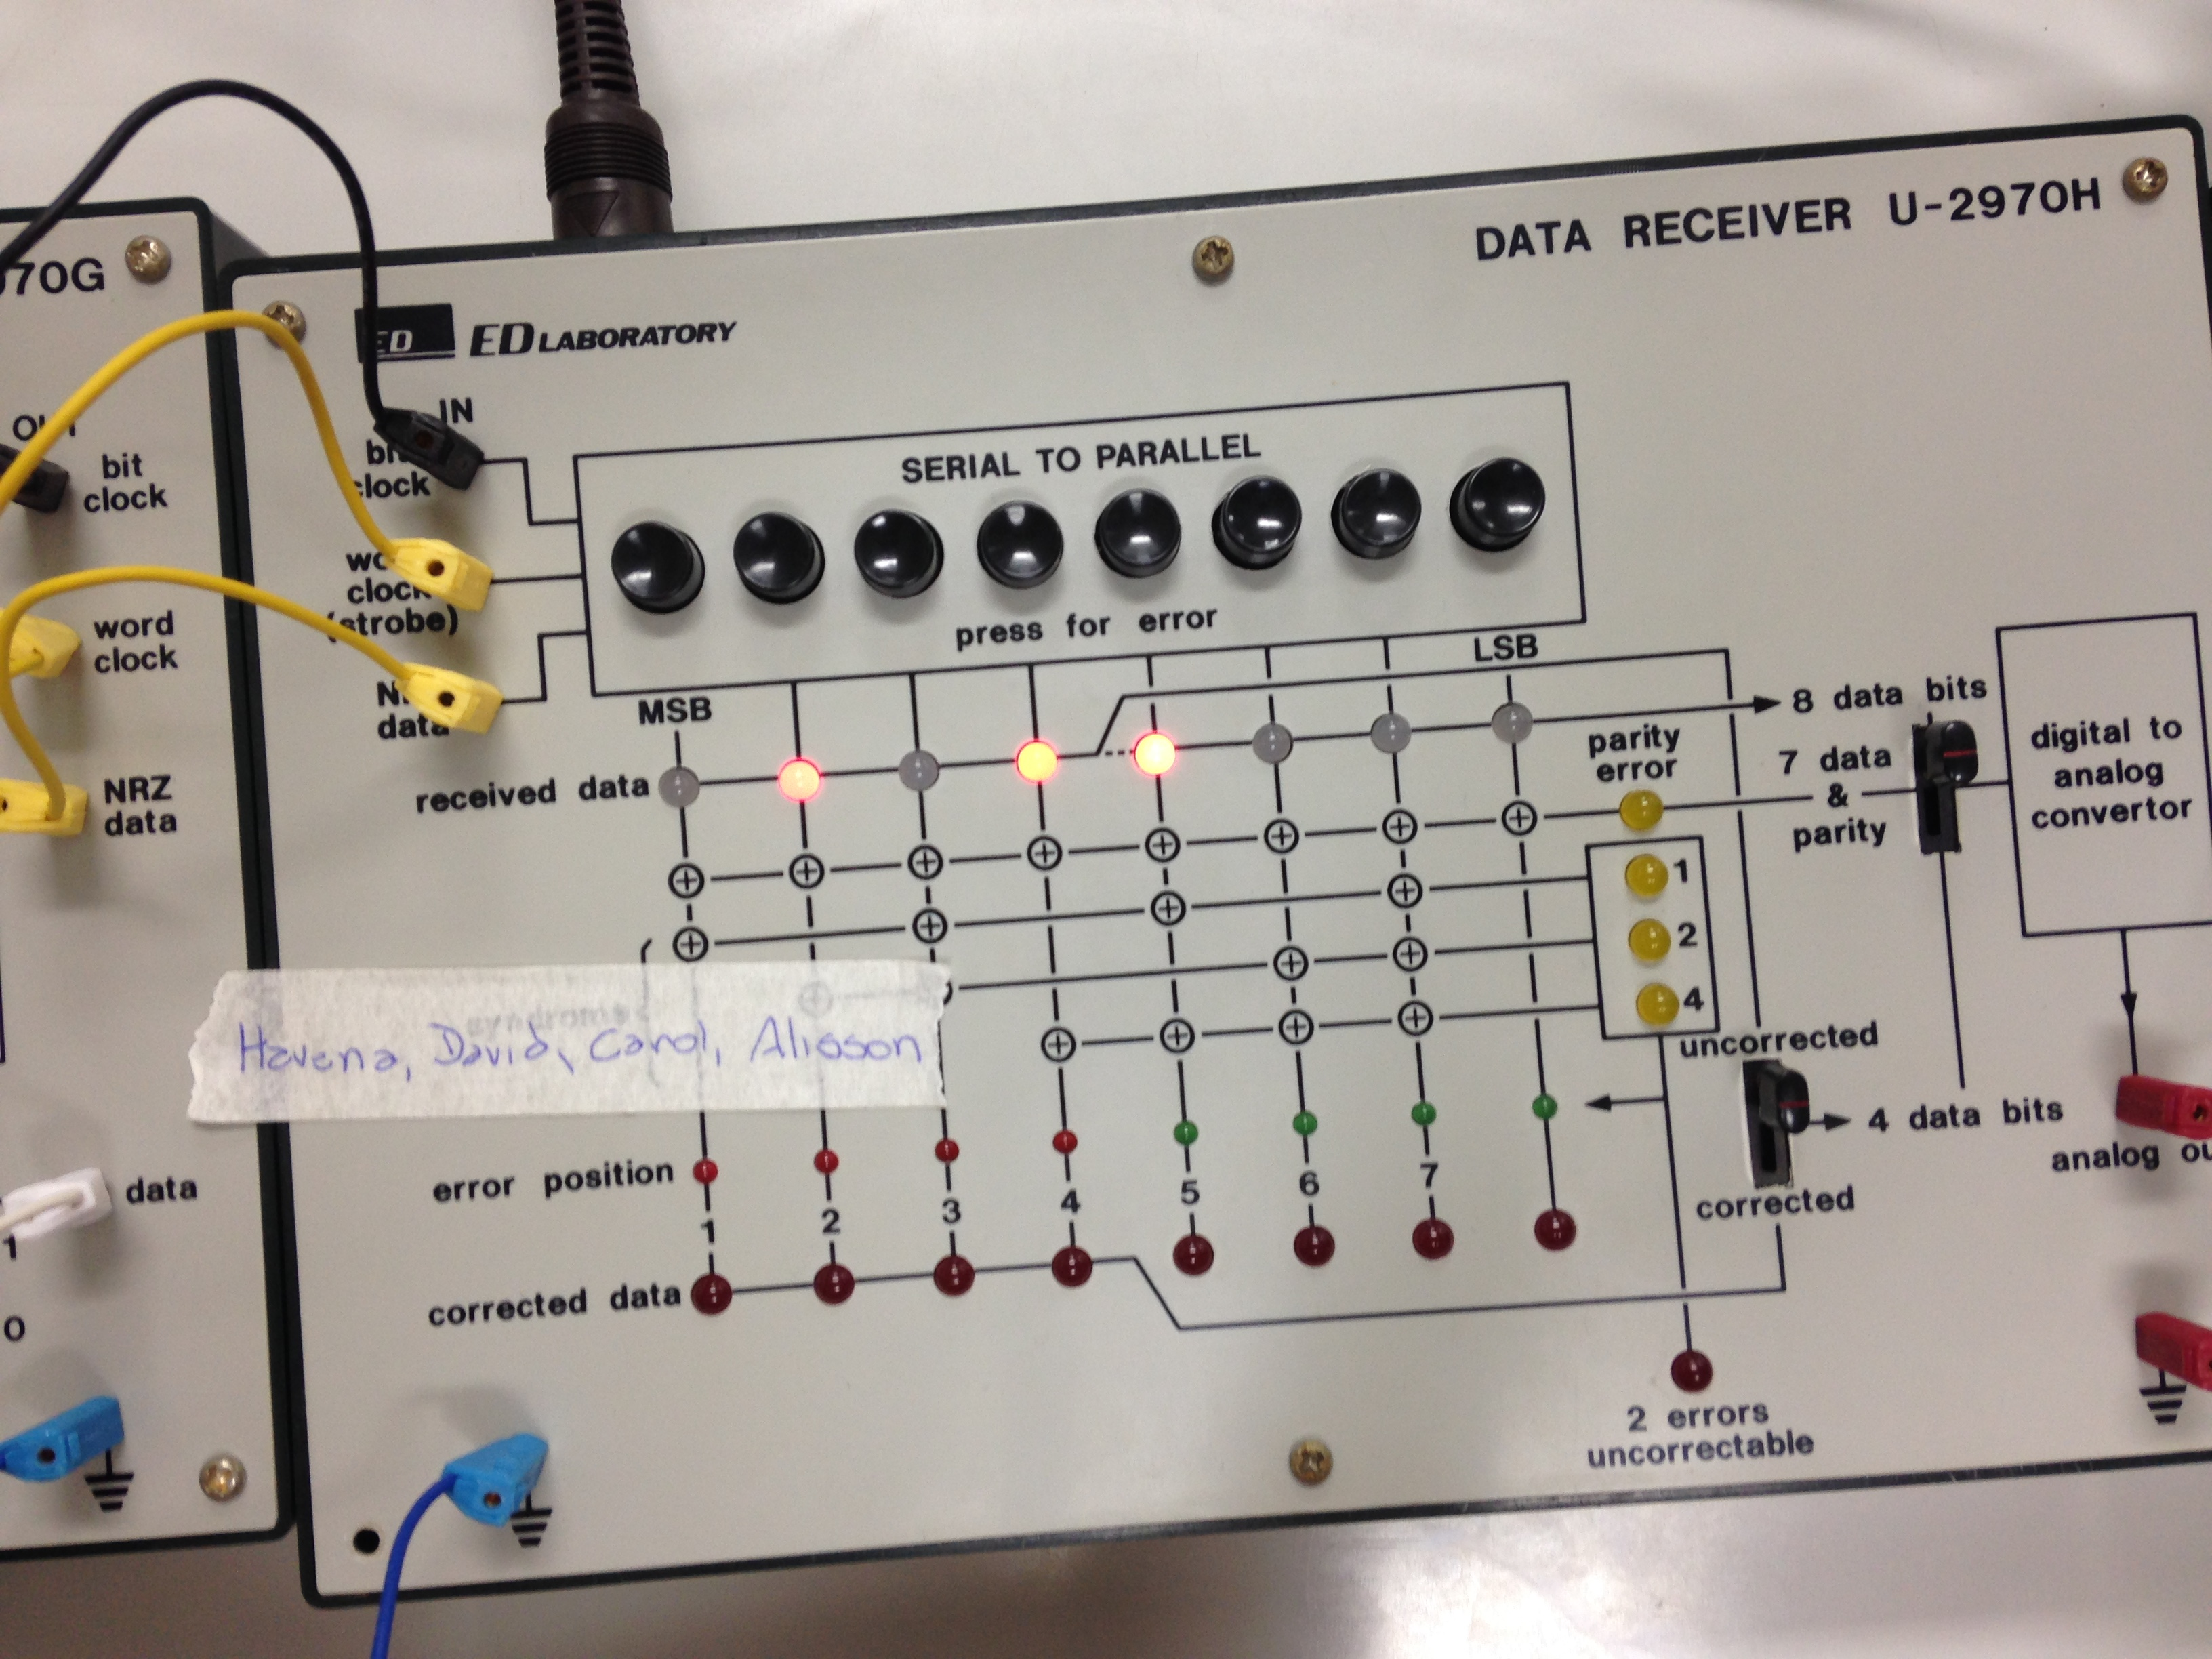
\includegraphics[scale=0.08]{f7}
			
		\small Fonte: Autoria própria.
		\label{fig:f7}
	\end{figure}
		

\subsection{Recuperação dos dados}

	A Figura \ref{fig:f8} foi obtida com a ponteira do canal 1 do osciloscópio na ligação 15. Nota-se a existência de grandes picos sobrepostos ao sinal semelhante ao sinal de entrada NRZ.
	
	\begin{figure}[H]
		\centering
		\caption{Picos sobrepostos.}
		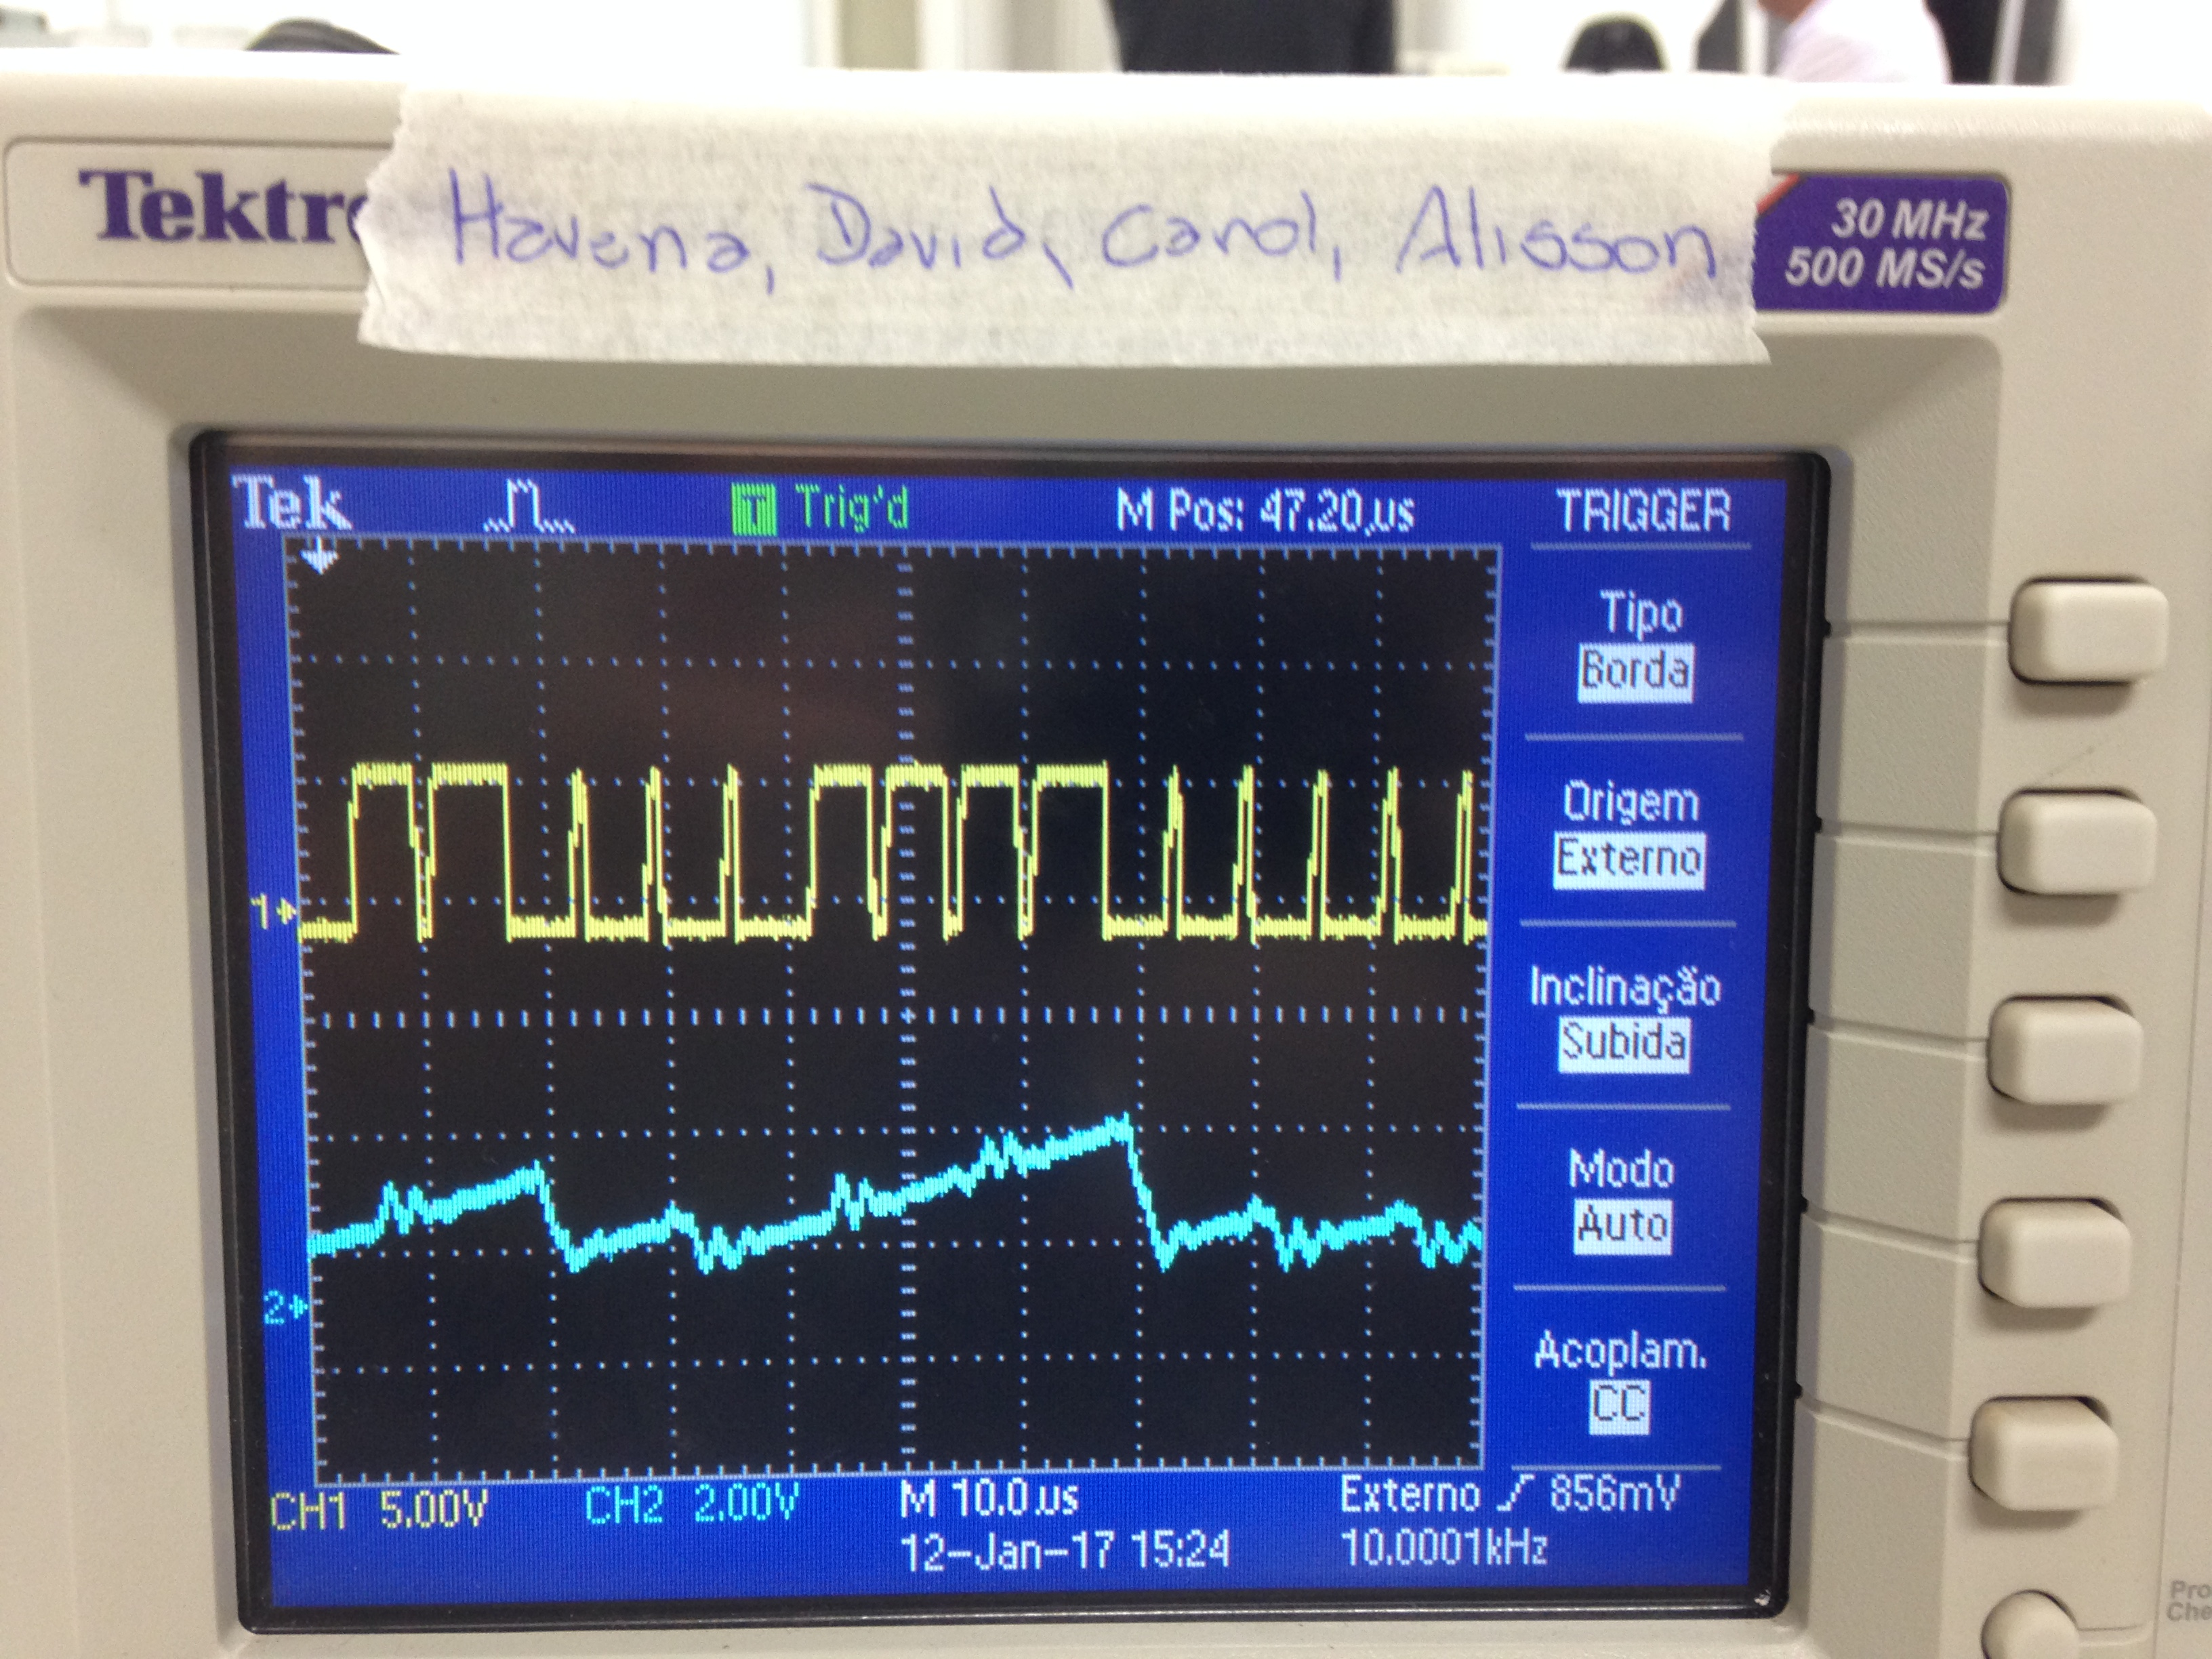
\includegraphics[scale=0.08]{f8}
			
		\small Fonte: Autoria própria.
		\label{fig:f8}
	\end{figure}
		
	Movendo o canal 2 do osciloscópio para a saída do integrador, foi observado que para um bit 0 a saída cresce durante o período de bit e para um bit de entrada 1, a saída decresce
	durante o período de bit, conforme mostra a Figura \ref{fig:f9}. Ao final do tempo de bit, o integrador é zerado.
	
	\begin{figure}[H]
		\centering
		\caption{Saída do integrador.}
		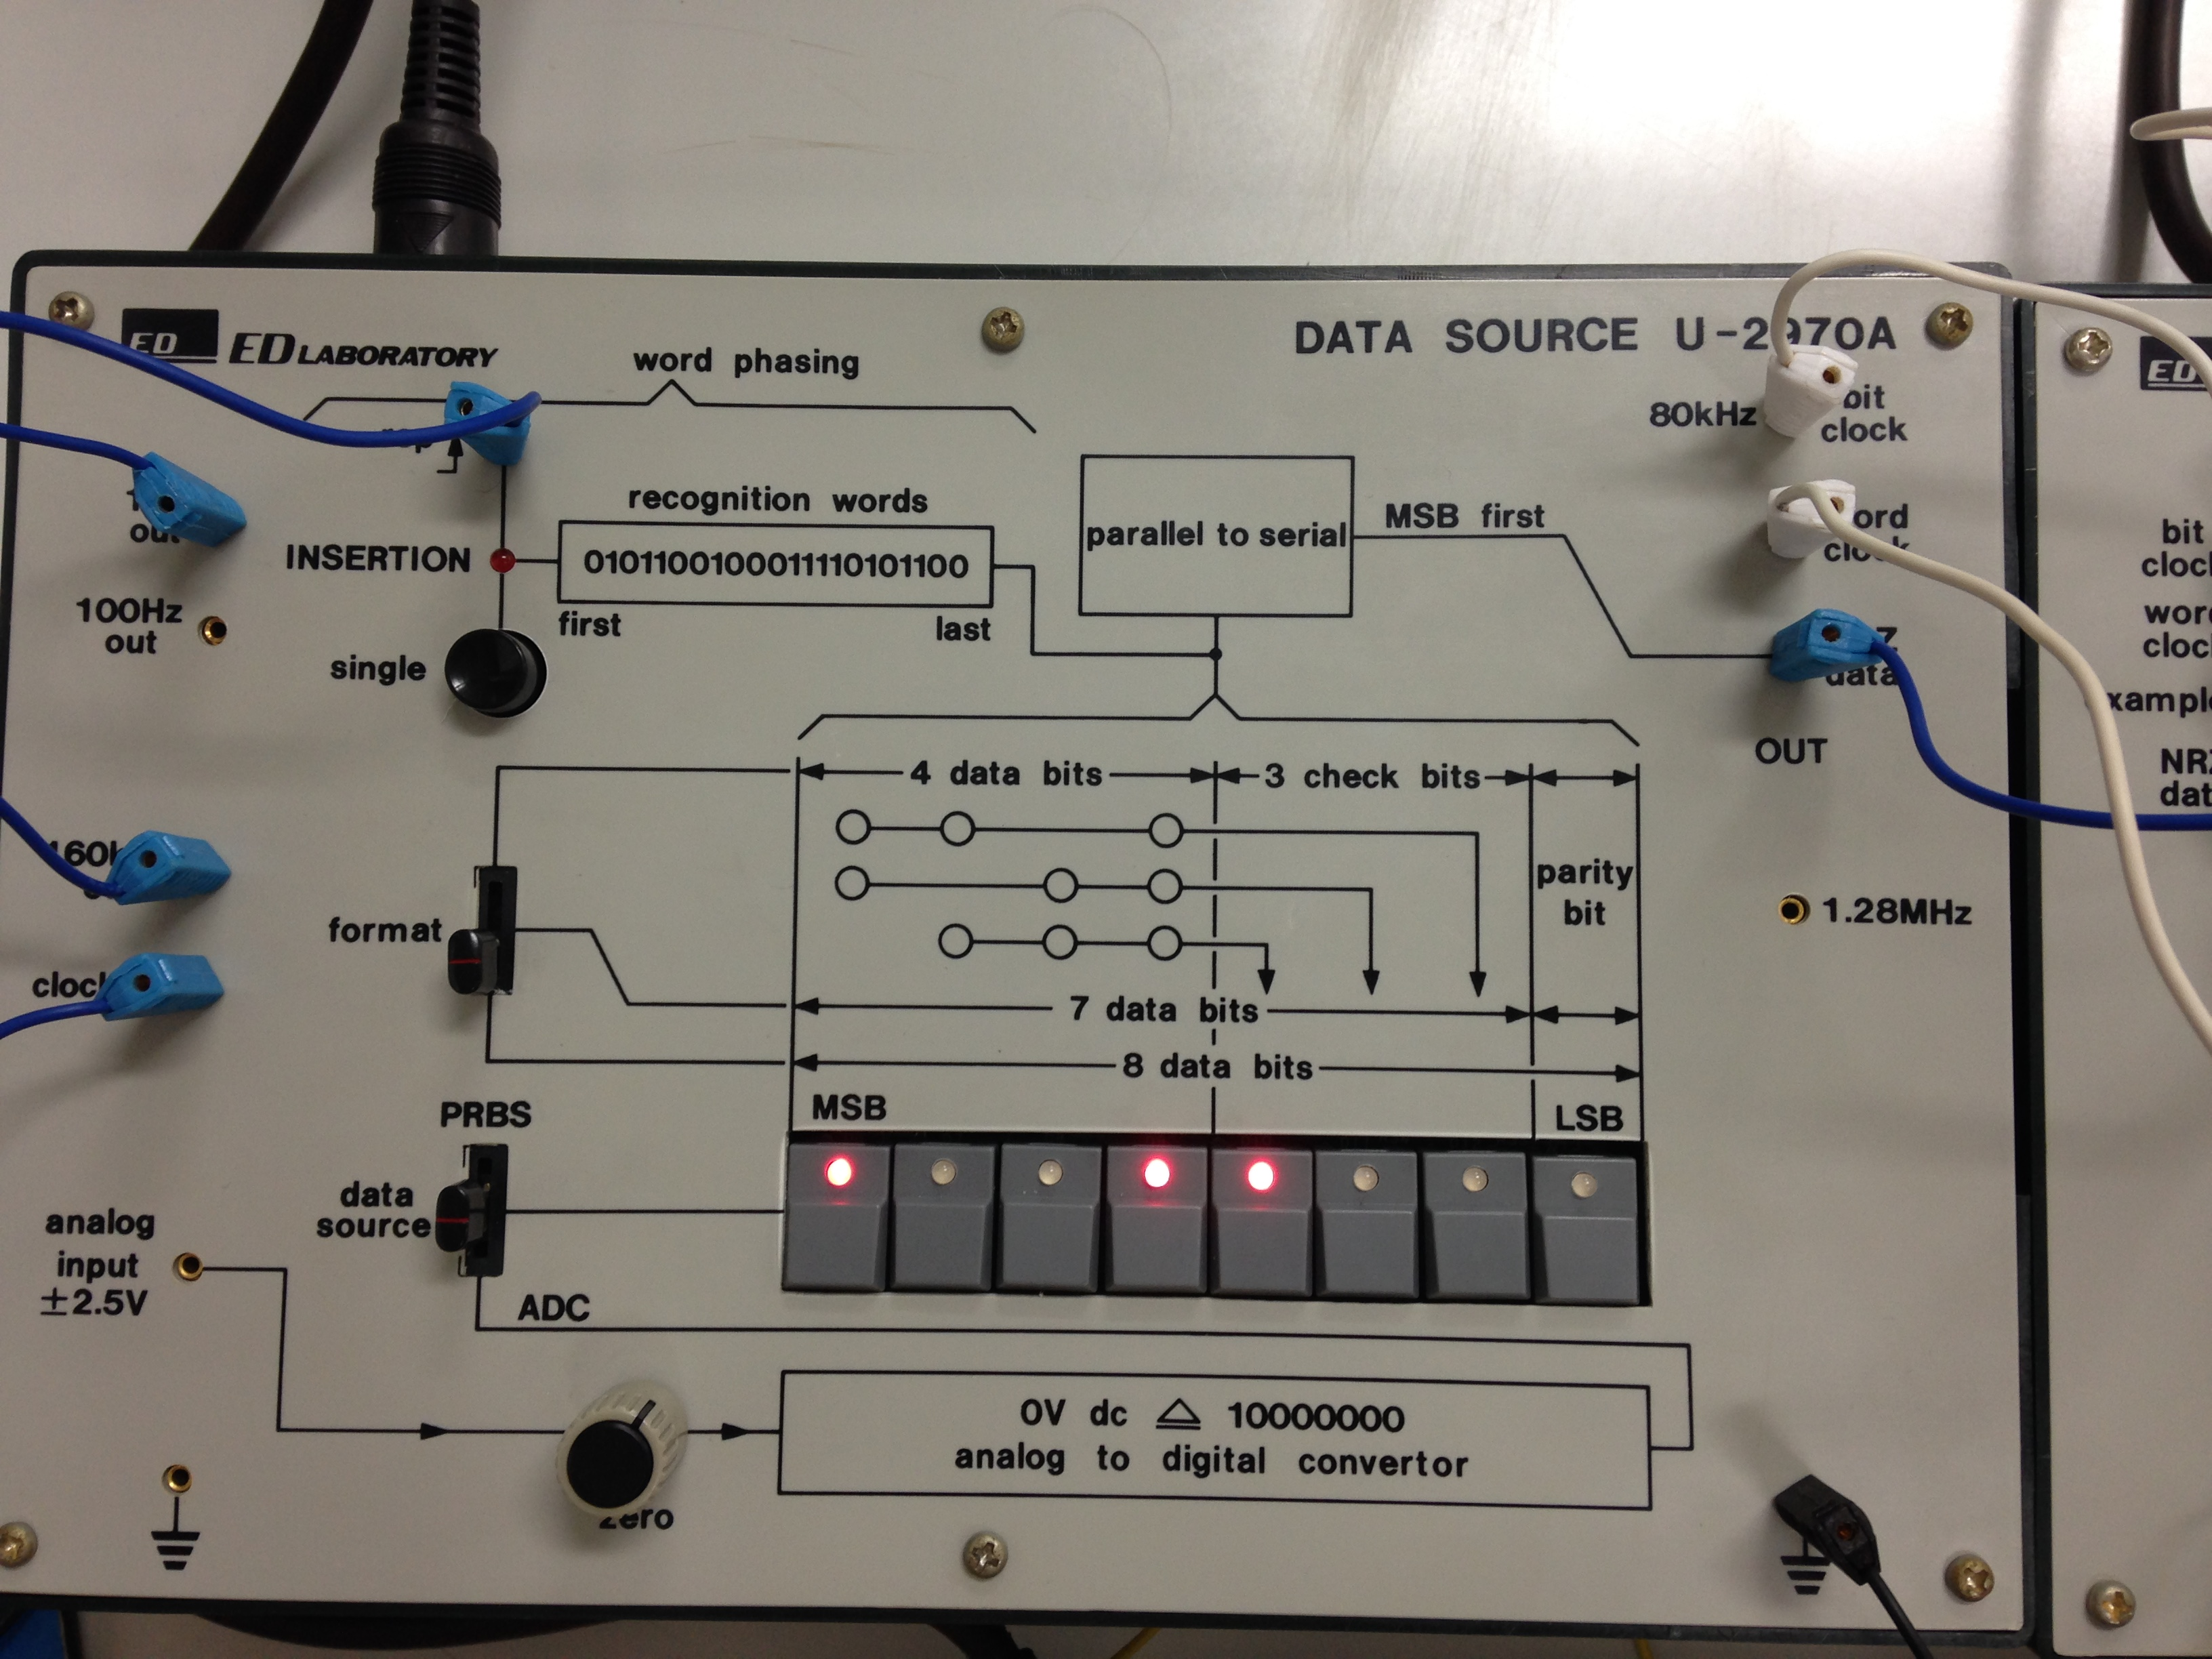
\includegraphics[scale=0.08]{f9}
			
		\small Fonte: Autoria própria.
		\label{fig:f9}
	\end{figure}
	
	Comparando o sinal de saída do canal 2 da Figura \ref{fig:f9} com o sinal do canal 1, os grandes picos do canal 1 são atenuados consideravelmente, exercendo pouca influência na saída do integrador.
	
	Ao observar os dados recuperados, fica evidente o atraso de um bit no sinal de saída, fato característico do processo de integração/decisão, conforme mostra a Figura \ref{fig:f12}.
	
		\begin{figure}[H]
			\centering
			\caption{Dados de entrada e dados recuperados.}
			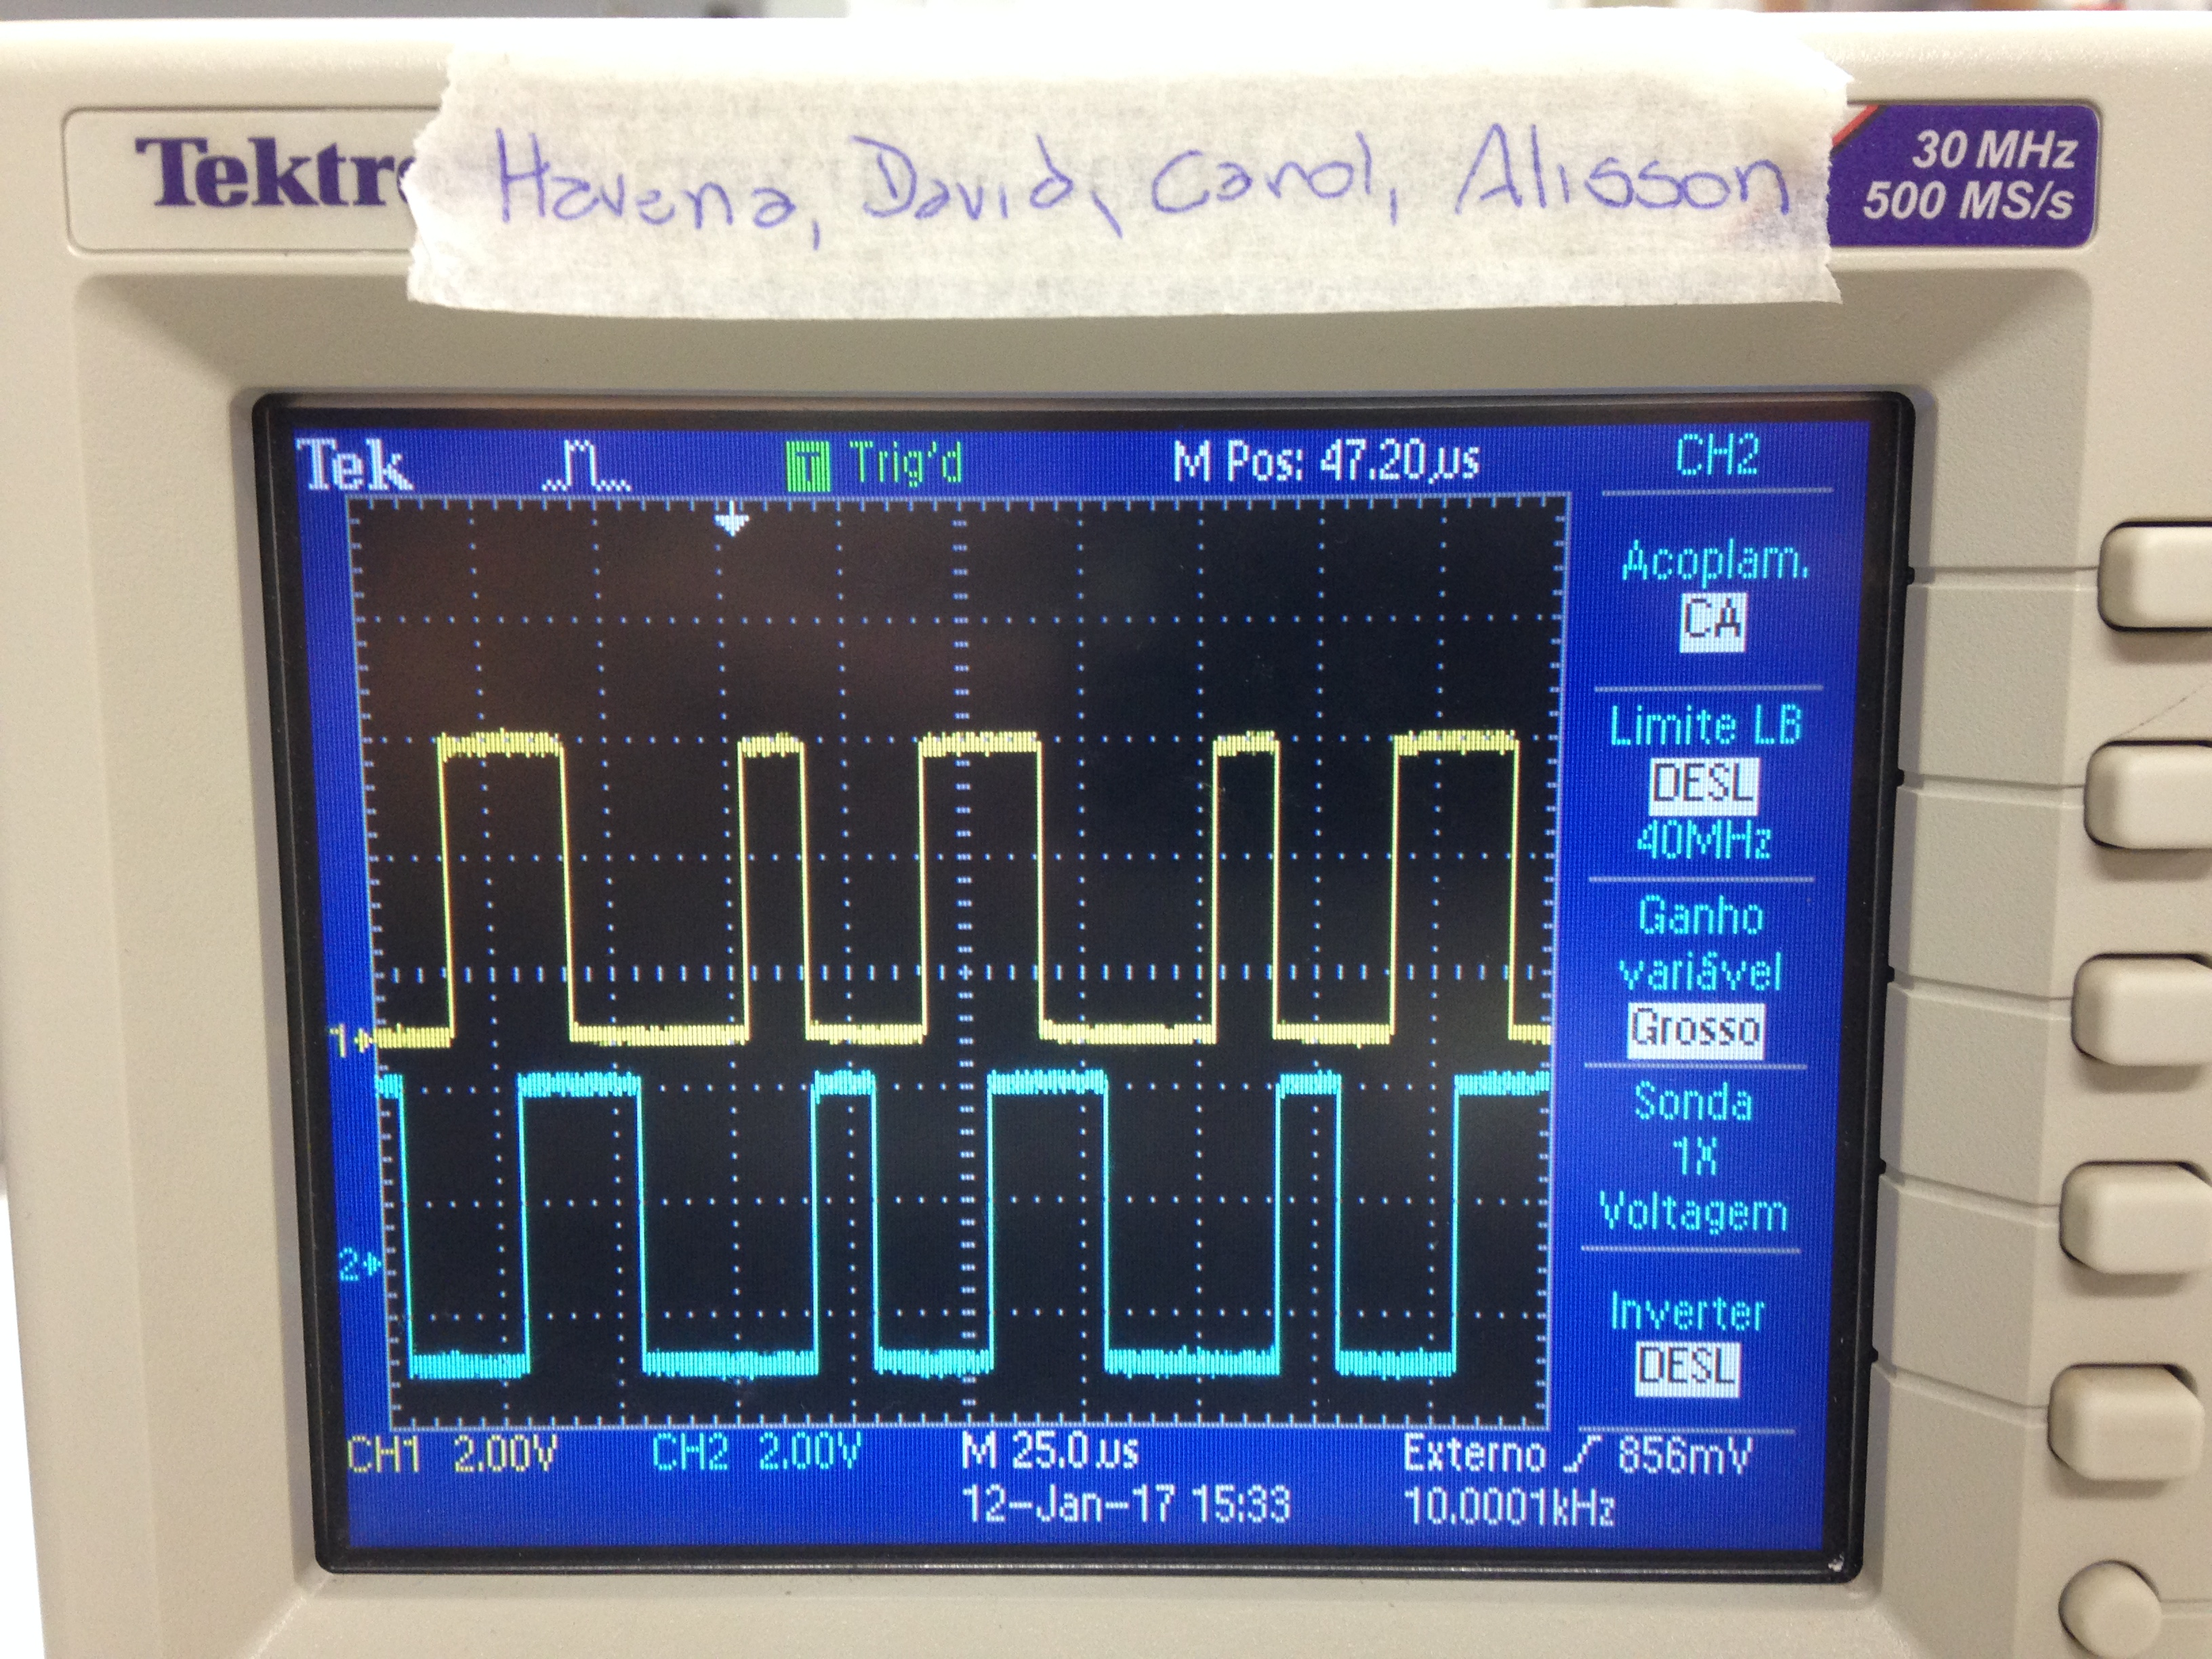
\includegraphics[scale=0.08]{f12}
			
			\small Fonte: Autoria própria.
			\label{fig:f12}
		\end{figure}


   
